\documentclass{sigchi}

% Use this section to set the ACM copyright statement (e.g. for
% preprints).  Consult the conference website for the camera-ready
% copyright statement.

% Copyright
\CopyrightYear{2020}
%\setcopyright{acmcopyright}
\setcopyright{acmlicensed}
%\setcopyright{rightsretained}
%\setcopyright{usgov}
%\setcopyright{usgovmixed}
%\setcopyright{cagov}
%\setcopyright{cagovmixed}
% DOI
\doi{https://doi.org/10.1145/3313831.XXXXXXX}
% ISBN
\isbn{978-1-4503-6708-0/20/04}
%Conference
\conferenceinfo{CHI'20,}{April  25--30, 2020, Honolulu, HI, USA}
%Price
\acmPrice{\$15.00}

% Use this command to override the default ACM copyright statement
% (e.g. for preprints).  Consult the conference website for the
% camera-ready copyright statement.

%% HOW TO OVERRIDE THE DEFAULT COPYRIGHT STRIP --
%% Please note you need to make sure the copy for your specific
%% license is used here!
% \toappear{
% Permission to make digital or hard copies of all or part of this work
% for personal or classroom use is granted without fee provided that
% copies are not made or distributed for profit or commercial advantage
% and that copies bear this notice and the full citation on the first
% page. Copyrights for components of this work owned by others than ACM
% must be honored. Abstracting with credit is permitted. To copy
% otherwise, or republish, to post on servers or to redistribute to
% lists, requires prior specific permission and/or a fee. Request
% permissions from \href{mailto:Permissions@acm.org}{Permissions@acm.org}. \\
% \emph{CHI '16},  May 07--12, 2016, San Jose, CA, USA \\
% ACM xxx-x-xxxx-xxxx-x/xx/xx\ldots \$15.00 \\
% DOI: \url{http://dx.doi.org/xx.xxxx/xxxxxxx.xxxxxxx}
% }

% Arabic page numbers for submission.  Remove this line to eliminate
% page numbers for the camera ready copy
% \pagenumbering{arabic}

% Load basic packages
\usepackage{balance}       % to better equalize the last page
\usepackage{graphics}      % for EPS, load graphicx instead 
\usepackage[T1]{fontenc}   % for umlauts and other diaeresis
\usepackage{txfonts}
\usepackage{mathptmx}
\usepackage[pdflang={en-US},pdftex]{hyperref}
\usepackage{color}
\usepackage{booktabs}
\usepackage{textcomp}
\usepackage{graphicx}

% Some optional stuff you might like/need.
\usepackage{microtype}        % Improved Tracking and Kerning
% \usepackage[all]{hypcap}    % Fixes bug in hyperref caption linking
\usepackage{ccicons}          % Cite your images correctly!
% \usepackage[utf8]{inputenc} % for a UTF8 editor only

% If you want to use todo notes, marginpars etc. during creation of
% your draft document, you have to enable the "chi_draft" option for
% the document class. To do this, change the very first line to:
% "\documentclass[chi_draft]{sigchi}". You can then place todo notes
% by using the "\todo{...}"  command. Make sure to disable the draft
% option again before submitting your final document.
\usepackage{todonotes}

% Paper metadata (use plain text, for PDF inclusion and later
% re-using, if desired).  Use \emtpyauthor when submitting for review
% so you remain anonymous.
\def\plaintitle{CSCM69: Human-Centred Perspectives and Methods\\Coursework 2 - Work/Life Balence}
\def\plainauthor{Andy Gray}
\def\emptyauthor{}
\def\plainkeywords{Authors' choice; of terms; separated; by
  semicolons; include commas, within terms only; this section is required.}
\def\plaingeneralterms{Documentation, Standardization}

% llt: Define a global style for URLs, rather that the default one
\makeatletter
\def\url@leostyle{%
  \@ifundefined{selectfont}{
    \def\UrlFont{\sf}
  }{
    \def\UrlFont{\small\bf\ttfamily}
  }}
\makeatother
\urlstyle{leo}

% To make various LaTeX processors do the right thing with page size.
\def\pprw{8.5in}
\def\pprh{11in}
\special{papersize=\pprw,\pprh}
\setlength{\paperwidth}{\pprw}
\setlength{\paperheight}{\pprh}
\setlength{\pdfpagewidth}{\pprw}
\setlength{\pdfpageheight}{\pprh}

% Make sure hyperref comes last of your loaded packages, to give it a
% fighting chance of not being over-written, since its job is to
% redefine many LaTeX commands.
\definecolor{linkColor}{RGB}{6,125,233}
\hypersetup{%
  pdftitle={\plaintitle},
% Use \plainauthor for final version.
%  pdfauthor={\plainauthor},
  pdfauthor={\emptyauthor},
  pdfkeywords={\plainkeywords},
  pdfdisplaydoctitle=true, % For Accessibility
  bookmarksnumbered,
  pdfstartview={FitH},
  colorlinks,
  citecolor=black,
  filecolor=black,
  linkcolor=black,
  urlcolor=linkColor,
  breaklinks=true,
  hypertexnames=false}

% create a shortcut to typeset table headings
% \newcommand\tabhead[1]{\small\textbf{#1}}

% End of preamble. Here it comes the document.
\begin{document}

\title{\plaintitle}

\numberofauthors{1}
\author{%
  \alignauthor{??\\
    \affaddr{??}\\
    \affaddr{Swansea, Wales}\\
    \email{??@swansea.ac.uk}}
}
\maketitle

\begin{abstract}
	one one one one one one one one one one one one one one one one one one one one one one one one one one one one one one one one one one one one one one one one one one one one one one one one one one one one one one one one one one one one one one one one one one one one one one one one one one one one one one one one one one one one one one one one one one one one one one one one one one one one one one one one one one one one one one one one one one one one one one one one one one one one one one one one one one one one one one one one one one one one one one one one one one one one one one 
	
\end{abstract}


% ACM Classfication

\begin{CCSXML}
<ccs2012>
<concept>
<concept_id>10003120.10003121</concept_id>
<concept_desc>Human-centered computing~Human computer interaction (HCI)</concept_desc>
<concept_significance>500</concept_significance>
</concept>
<concept>
<concept_id>10003120.10003121.10003125.10011752</concept_id>
<concept_desc>Human-centered computing~Haptic devices</concept_desc>
<concept_significance>300</concept_significance>
</concept>
<concept>
<concept_id>10003120.10003121.10003122.10003334</concept_id>
<concept_desc>Human-centered computing~User studies</concept_desc>
<concept_significance>100</concept_significance>
</concept>
</ccs2012>
\end{CCSXML}

\ccsdesc[500]{Human-centered computing~Human computer interaction (HCI)}
\ccsdesc[300]{Human-centered computing~Haptic devices}
\ccsdesc[100]{Human-centered computing~User studies}

% Author Keywords
\keywords{\plainkeywords}

% Print the classficiation codes
\printccsdesc
Please use the 2012 Classifiers and see this link to embed them in the text: \url{https://dl.acm.org/ccs/ccs_flat.cfm}



\section{Introduction}
	Harvard conducted a survey which asked professional people how many hours they worked a week, 94\% said they put in more than 50 hours or more. Out of these professionals, 50\% said they are working 65 or more hours \cite{harvard_review}. What is even more staggering is that this survey got done in 2009, a time where Blackberry mobile phones were all the rage and iPhones had only been on the market for around two years. This year was when the iPhone 3G was just about to hit stores and was way before the iPhone 4 and where the smartphone, as we currently know them, indeed took off and changed the way we interact with our mobile devices. As the Harvard survey also found out that 20-25 hours a week get spent monitoring their Blackberrys while outside of working hours \cite{harvard_review}. 
	
	
	These numbers show that a work-life balance has been an issue for some years. Especially when looking at statistics published in 2020, by the NY Post's Business Insider, that state 48\% of Americans consider themselves workaholics and the CNBC stating that 66\% of American works lacking a healthy work-life balance \cite{work-life_2020}. A staggering fact that we can relate to from experience is that 77\% of full-time works suffer from burnout from their current job \cite{work-life_2020}. Rescue Time analysed their users' data in 2019 and found that 40\% of people used their computers after 10 pm and 28\% of people start their workday before 8:30 am \cite{rescuetime_study}.  
	
	What we aim to do within this report is to identify some of the leading apps that get associated with work-life balance. Once these apps get identified, we aim to investigate these tools while critiquing their designs concerning their interactions with HCI. These apps include \textbf{[list apps here]}, we will then be interviewing users and finding out their views on these applications and how they have impacted their work-life balance.
	
	%[Overview of the assignment]
	  

\section{Existing apps and devices used Widley in Work-Life Balance}
	% Find out what key existing apps, services and devices are widely used in the domain of interest that you have chosen. For example, this might include fitness trackers, creativity support apps or other domain-specific services. As a guide, I would expect you to find around 3–5 tools here.
	
	"With the pervasiveness of technology, it has not only permeated our workspaces but it has also become invasive in our private personal spaces \cite{peters2012sig}." This quote got taken from a CHI paper published in 2012. In this paper, they state what defines a work-life balance is on the worker working longer than 50 hours a week compared to personal care and leisure whether it gets paid, or unpaid, but for women that also include the rate of employees who have children \cite{peters2012sig}. With this definition in mind, we are going to identify and critique four apps and devices that have made an impact for good and bad reasons for people's work-life balance. The applications and devices we will be looking at are emails, instant messaging (IM), meditation apps and mobile phone devices.
	
	%Email
	One application that has brought about both good things and bad things for work-life balance is the email. While it made communication more accessible, especially in the early days as we did not have to wait for a letter to get sent in the post, it has now become very consuming. In result, it has created a sense of urgency around reading and responding to emails straight away \cite{stawarz2013d}. However, in terms of work, email has improved the efficiency of working when aiming to communicate with colleges or other people when they are not physically present.
	
	%IM
	An application that has both a positive and negative effect on work-life balance is instant messaging, for example, WhatsApp, iMessage, Facebook Message, Slack. IM has shown how the same communication channel often gets used personal activities and work arrangements. In some cases, both personal and work activities get almost done at the same time \cite{lindley2012s}. However, IM has become an alternative method to the traditional communication methods for both work \cite{siggroup2005group} and private communication \cite{flanagin2005online}, instead of it being an additional medium on top. However, IM, by its very definition, is an interruption, especially if we use the definition defined by O'Conaill \& Frohlich, "a synchronous interaction which is not initiated by the recipient, is unscheduled, and results in the recipient discontinuing their current activity" \cite{rennecker2003theorizing}. 
	
	%Meditation Apps
	In the hustle and bustle of the modern-day life, especially while at the time of writing being in a second national lockdown in the UK and a global pandemic happening, public's perception around mental health has started to shift focus. Applications that get promoted to help with mental health and lockdown are meditation apps. While mindful apps do help with well being and mental health, however, they require training in order to be completely effective \cite{dauden2018evaluating}.  Mindfulness gets defined as the "awareness that arises through paying attention on purpose, in the present moment without judgment \cite{baer2003mindfulness}". A study of mindful applications has found that only 4\% provide any form of mindfulness training, the rest only offer time reminders for doing meditation \cite{mani2015review}. 
	
	%Mobile
	The one technology that has made both work-life better and worse at the same time, depending on what angle it gets looked at is the mobile phone. Through the introduction of mobile phones, it has made it very difficult to separate work-life \cite{gronvall2016hci, sadler2006balancing} as all the previous apps have demonstrated. This issue is a result of the mobile phone being the one device that enables all of these. Mobile phones have created a grey area between private and work domains, which is why much research is getting carried out in this area \cite{fleck2015balancing}. As studies have shown that Workers average just 2 hours and 48 minutes of productive device time a day and check emails and IM about every 6 minutes on average \cite{rescuetime_study}. We wonder if this is a result of mobile phones and them being so available and accessible to "just check" at any points.
	
	\section{Critiquing Existing Apps and Devices for Work-Life Balance}
	
	We will now be critiquing existing apps and devices within the areas that we have identified as widely used within the work-life balance. We will be identifying one app or device, within the different areas, and then critiquing them, aiming to identify how they could be adapted to amplify the user's experience. We will be looking at how the app or device makes it a particular part of being human, and how they aim to do this and possibly how they could do it better.
	
		\subsection{Mobile Phones (Device)}
		% Critique the device
		% Have work/life modes - like light or dark mode.
		Mobile devices have been around for many years until the introduction of the smartphone, that we know today, laptops were the only primary way to do any form of real work on the go. However, these did have their limitations and their pros. However, since the introduction of smartphones, and how powerful and capable they now are, mobile devices and the ability to do work from them has increased and become more proficient. While there are many smartphone devices out there, we will be focusing on Apple's iPhone for our critique. We have chosen this device primarily due to our more familiarity with the device and what it can do. 
		
		The mobile device, in the modern-day, is an essential item for most people. People use them for a while range of things, whether it be for socialising, relaxing by play games, for example, or get used for business. No one device has given the user so much freedom in what it can allow to user to do before, while still be relatively small and can be carried in just a pocket. However, the applications and features that enable us to do so much. They can and do get used for so much more than what its intention was. For example, social media intended to connect people around the world if we take Facebook in this case. However, it has now not only become a platform to allow people to communicate, but it has allowed the business to have a platform to be able to trade from that would not have been their before. So social media is also business media, or is still social media? As we can see, a vast grey area has got generated, which we believe through mobile phones to how accessible they are and how they connect to the internet 24/7 unless the user has run out of data allowance, and world wide web. However, this ability to have so much content on-demand, we could say, has created a form of addiction but this could be down to their interruption nature, through notifications and attention-grabbing features like ringtones, and haptic vibrates. So with mobile phones getting used for social and work, is there any surprise that works are not super productive within a typical workday or struggle to switch off from work. While we have used social media as an example, in this case, it is valid for several different applications available, like emails, instant messaging and socialising. We believe as they are all in one place, it has made it harder to maintain an excellent work-life balance.
		
		\subsection{Email}
		% Critique the app
		
		
		\subsection{Mindful Application - Calm}
			% https://usabilitygeek.com/ux-case-study-calm-mobile-app/
		
		\subsection{Whats app / (Instant Messaging)}


\section{Investigate these tools, critiquing their design}
		\subsection{Mobile Phones (Device)}
		\subsection{Smart Watch (Device)}
		\subsection{Email}
		\subsection{App timer notifiers - think apple screen time.}
	
	

%\begin{figure}
%	\begin{center}
%		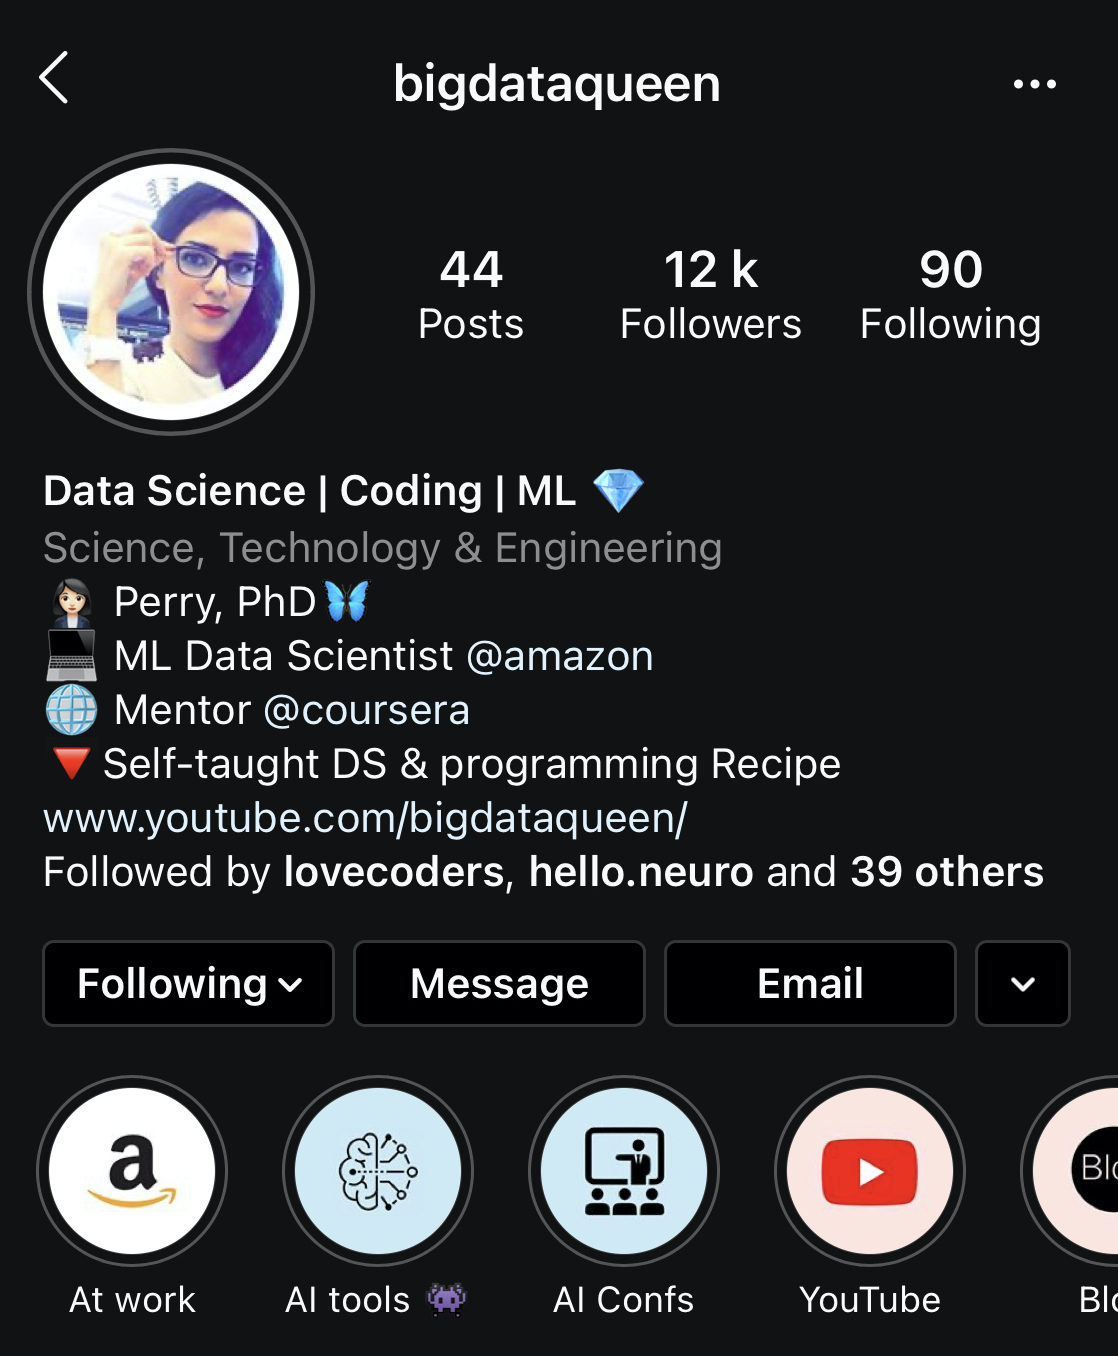
\includegraphics[width=5cm]{instagram_example2.jpeg}
%		\caption{An Instragram user profile overview. This is @bigdataqueen public profile overview.}
%		\label{fig:instagram_overview}
%	\end{center}
%\end{figure}


\section{Design an User Study? -> That what its called?}
	explain what will be included int he US and why made choices?

%\begin{figure}
%	\begin{center}
%		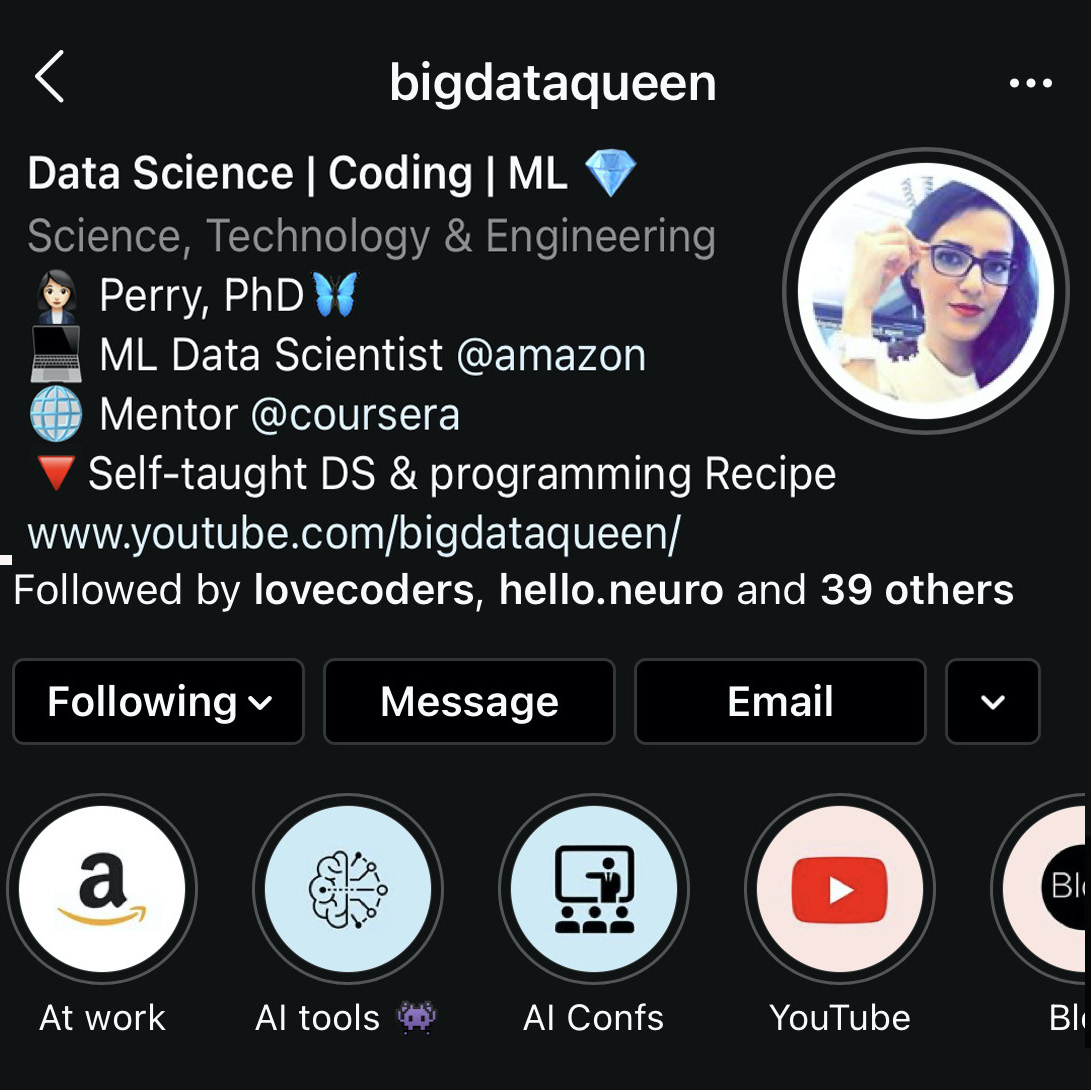
\includegraphics[width=5cm]{instagram_example2.jpg}
%		\caption{A design concept of @bigdataqueen new public profile overview.}
%		\label{fig:instagram_new_overview}
%	\end{center}
%\end{figure}

	


\section{Write up your results}
	place the results here in tables etc and discuss about them.

\section{Conclusion}
	 
	
	
% BALANCE COLUMNS
\balance{}

% REFERENCES FORMAT
% References must be the same font size as other body text.
\bibliographystyle{SIGCHI-Reference-Format}
\bibliography{sample}

\end{document}

%%% Local Variables:
%%% mode: latex
%%% TeX-master: t
%%% End:
